% Chapter Template

\chapter{Scaffold} % Main chapter title

\label{Chapter7} % Change X to a consecutive number; for referencing this chapter elsewhere, use \ref{ChapterX}

 %----------------------------------------------------
 
 

The scaffolds are three-dimensional supports that provide cells with an environment to adhere to, differentiate and multiply. Tissue engineering and scaffolds have been developed with the aim of promoting the regeneration of damaged tissues of the body, replacing the \emph{autologous grafts} and \emph{donor transplants}. \\ Autologous grafts example of skin or bone) require further surgery to be taken; furthermore, the tissue to be taken could be present in quantities not sufficient to the needs of regeneration of the damaged site. As regards the homologous grafts (from donor of the same species) the most important problems concern the lack of donor material and the biological risk of infection and rejection. \\
To provide the best environment for each group of cells grown, scaffolds made from a wide variety of materials have been described. Each fabric is in fact unique for mechanical and functional properties, as well as for its micro and macrostructure. \\ The introduction of additive manufacturing techniques in the production of scaffolds has brought novelty in the materials used and combinations of these, and has made it possible the exploration of alternative designs. The scaffolds can be made of biological polymers, synthetic polymers, ceramic materials and combinations of these \parencites{Reference128}. \\
The spread of cells and nutrients and the removal of waste substances must be facilitated by the scaffold structure to promote cell survival. The \emph{porosity} of the scaffold is therefore a fundamental parameter, along with the \emph{porosity interconnection}. Growth factors and regulatory proteins of cell adhesion can be integrated into scaffolds, to facilitate cell distribution and regulate it in the case of \emph{scaffold multipase} \parencite{Reference129}. The scaffold must also be reabsorbable, and the rate of reabsorption must be in accordance with the regeneration rate of the fabric to be repaired; the goal of the scaffolds is indeed to stimulate the complete regeneration of the fabric, with the total disappearance of the scaffold from the implant site. \\
Among the most recently used dental scaffolds we find ceramics granules such as \emph{tricalcium phosphate} (TCP, TriCalcium Phosphate), \emph{Hydroxyapatite} (HA) and MTA. These materials are used for bone regeneration, along with the collagen or PTFE membranes used to compartmentalize the graft site. The ceramic granules form a porous structure that is held together by the coagulum, promoting the spread of cells and nutrients and stimulating bone production. \\ The chemical composition of these granular materials is similar to that of bone, the high roughness surface allows the stabilization of the clot, the adsorption of growth factors and increased cell adhesion. The porosity of the materials described is not controllable, because it depends on the aggregation that is created during the formation of the blood clot. The resulting clot is also unstable and unsuitable to support mechanical loads during the early consolidation steps \parencite{Reference131}. The rate of reabsorption of some of these materials is slow, so they often find themselves in the site for a long time.
The use of three-dimensional scaffolds has therefore tried to overcome these limitations, trying to provide an optimal solution to these problems and to increase the predictability of the regenerative treatment. The introduction of additive manufacturing has made it possible to have greater control over the scaffold architecture, leading to very encouraging results \parencite{Reference136}, \parencite{Reference137}.\\
\begin{figure}[h]
\vspace{-10pt}
	\begin{center}
	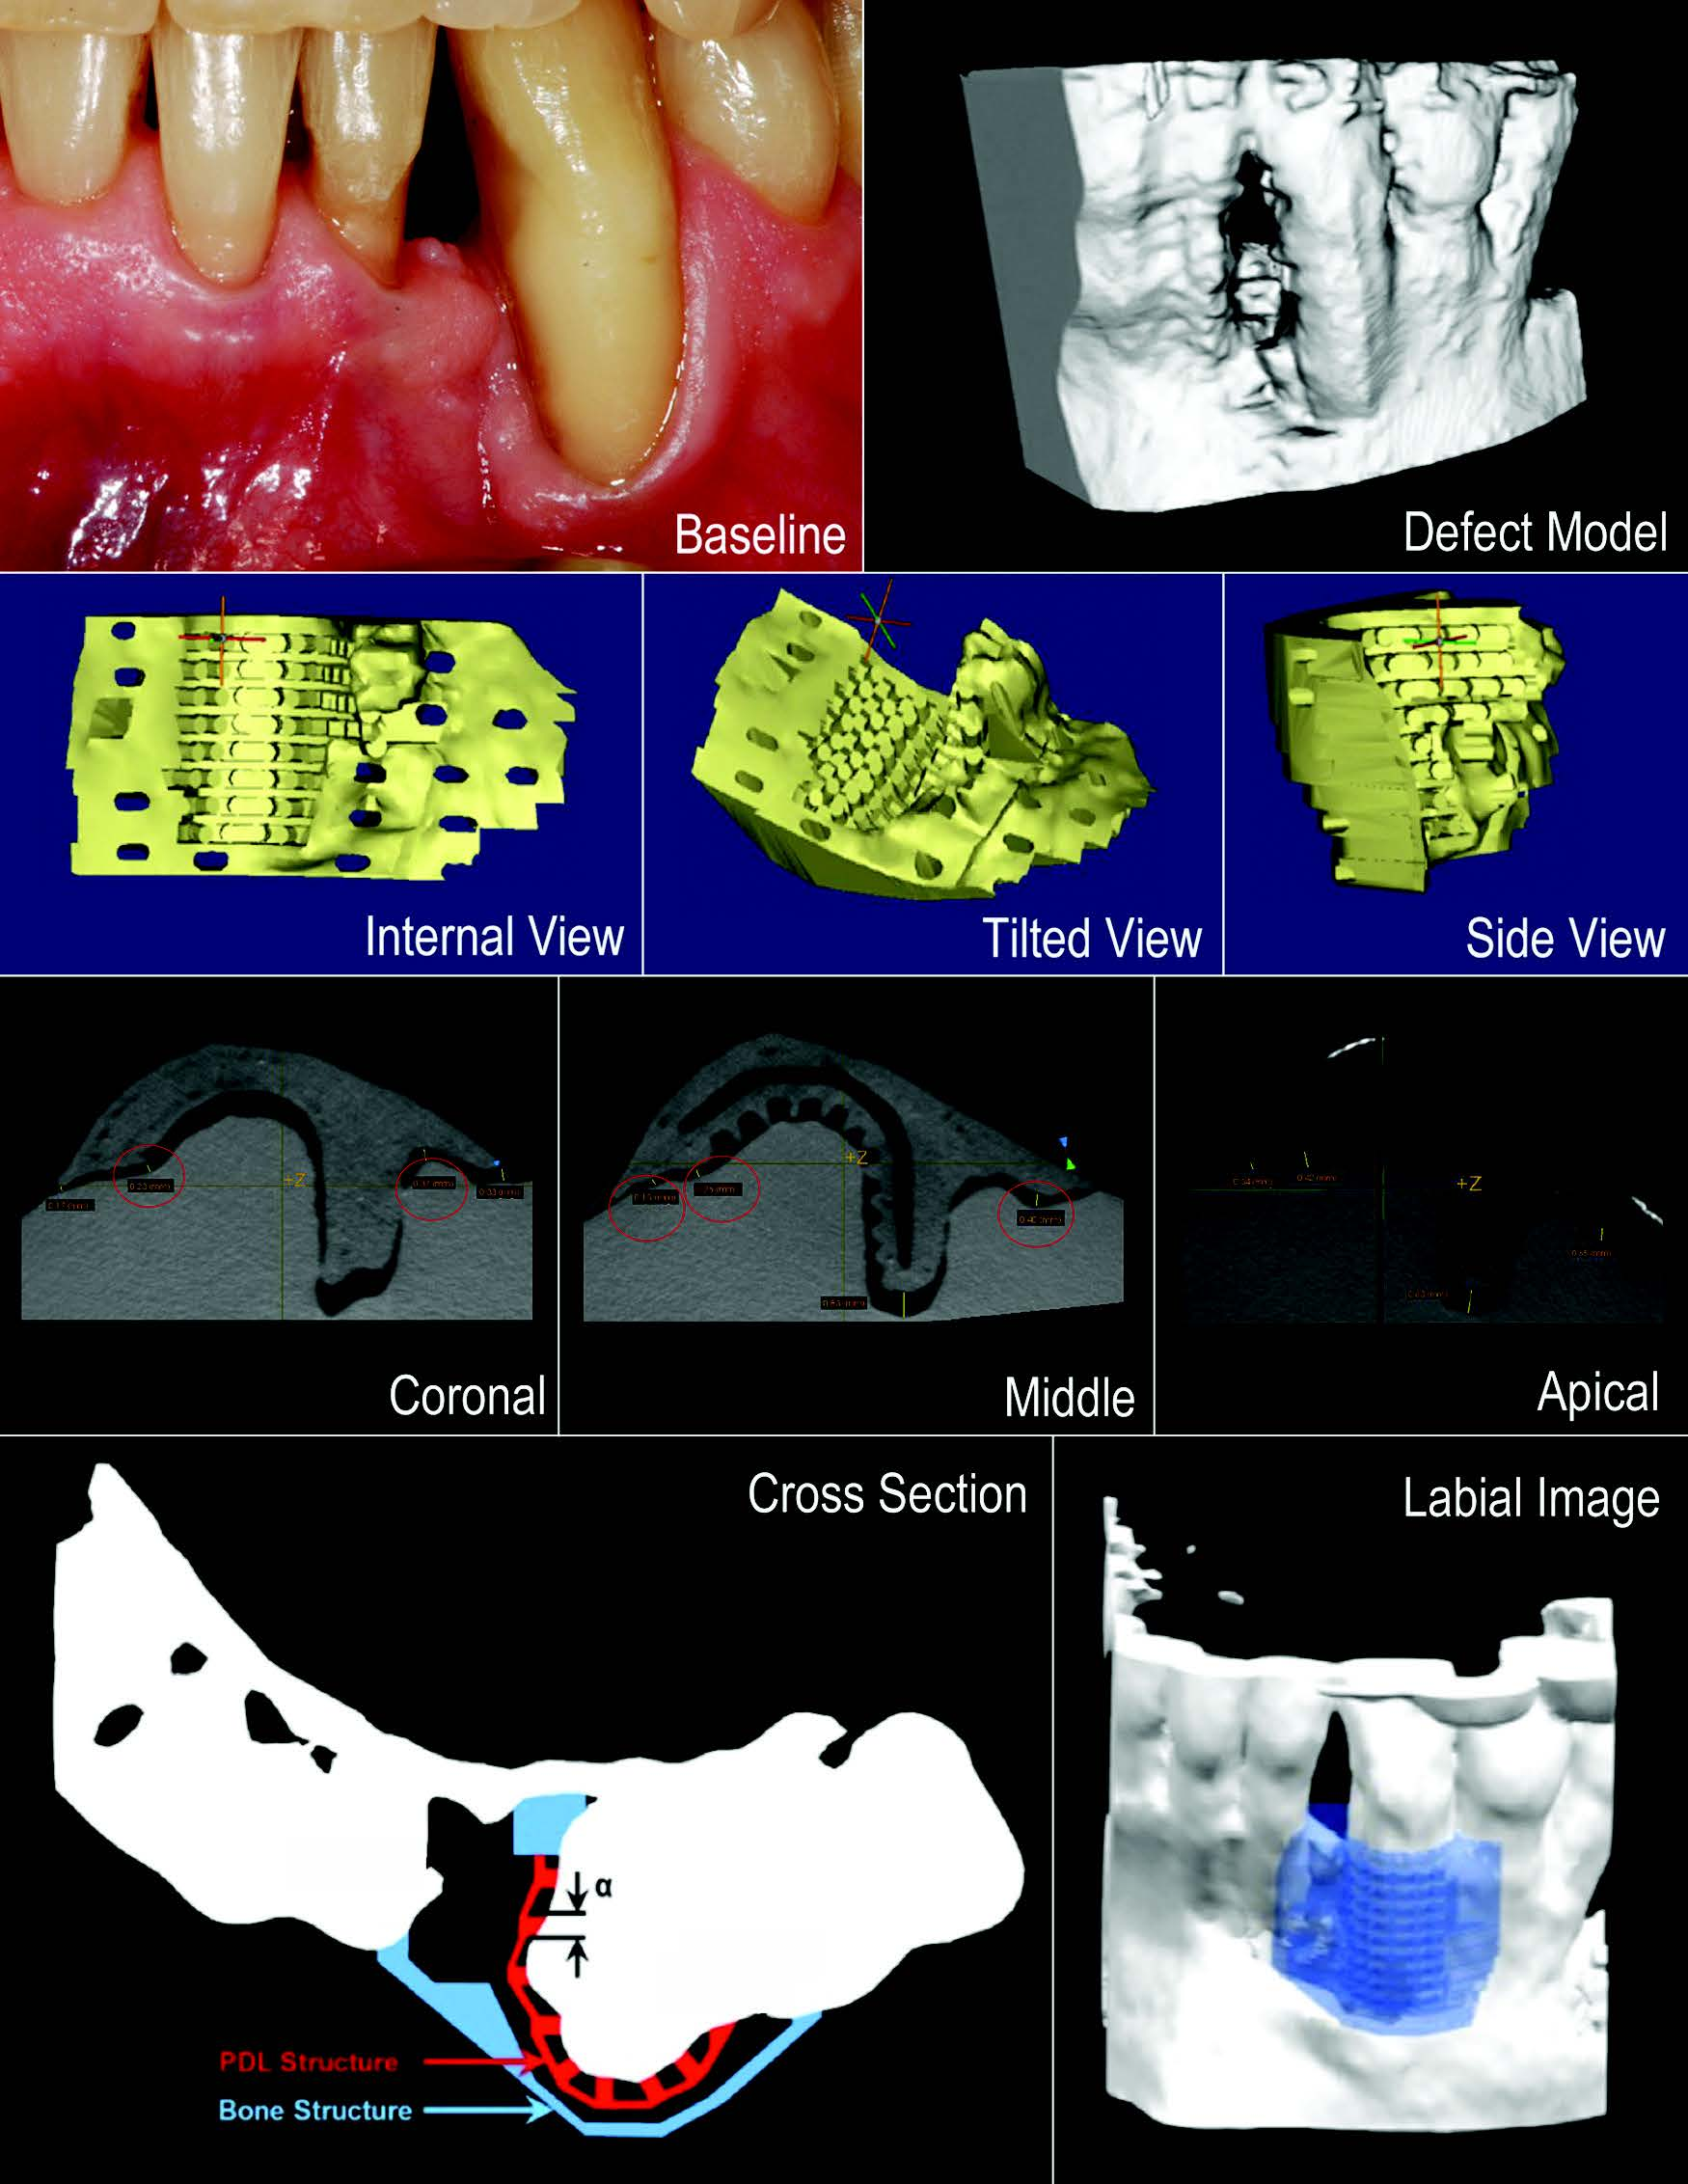
\includegraphics[width=0.6\textwidth, keepaspectratio]{scaf_paro}
    \caption{Scaffold per la rigenerazione parodontale realizzato da \emph{Rasperini et al} \parencite{Reference134}.}
    \label{fig:scaf_paro}
	\end{center}
\vspace{-20pt}
\end{figure}

Structures in OCT (\emph{occhocalcic phosphate}) result in \emph{\ textbf {ostoinduttive}}, that is, they stimulate the cells to osteoblastic differentiation \parencite{Reference130}. Osteoinductive has also proved to be a composite scaffold made of polycaprolactone and decellularized bone \parencite{Reference132}. A bioactive hydrogel composed of alginate, gelatin and OCT (56, 14, 30 wt\%, respectively) containing Vancomycin or Doxorubicin was tested in order to realize scaffolds with \emph{antibacterial} and \emph{antitumorals} properties, with results interesting \parencite{Reference133}. \\
Lastly, the recent attempts to realize three-dimensional scaffolds for the periodontal ligament regeneration are promising. The periodontal regeneration requires reconstitution of alveolar bone, periodontal ligament and dental cement, so the classic concept of compartmentalisation of the periodontal defect has been extended with the use of three-dimensional anisotropic scaffolds, with different compartments and geometric and structural characteristics related to the specific tissue to regenerate, such as the guides to direct the regeneration of periodontal fibers. \\
Several authors have made this type of scaffold, and in one case this was tested on the patient, but was then removed after 13 months by exposure of the same in oral cavity \ref{fig:scaf_paro}. Slowness in the degradation of the material and the reduced porosity of the scaffold have been shown to be primarily responsible for the failure \parencite{Reference134}. \\
\begin{figure}[h!]
 
\begin{subfigure}{0.5\textwidth}
\centering
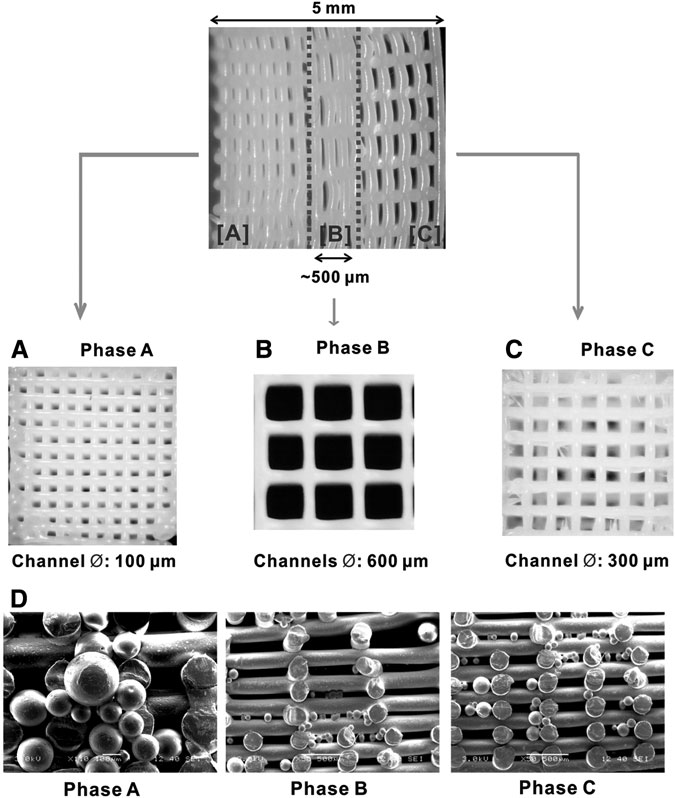
\includegraphics[width=\linewidth, keepaspectratio]{trifase} 
%\caption{}
\label{fig:trifase}
\end{subfigure}
\begin{subfigure}{0.5\textwidth}
\centering
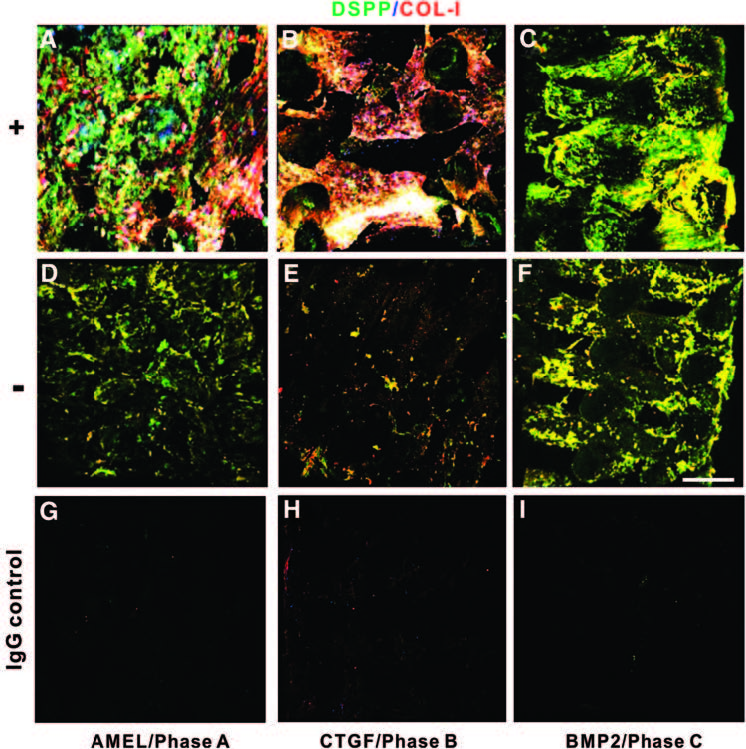
\includegraphics[width=\linewidth, keepaspectratio]{histo}
%\caption{}
\label{fig:histo}
\end{subfigure}
\caption{\textbf{A sinistra}: \emph{scaffold trifase} per la rigenerazione del complesso parodontale con microsfere contenenti fattori di crescita. \emph{\textbf{Phase A}}: scaffold per la rigenerazione del cemento radicolare; \emph{\textbf{Phase B}}: scaffold per la rigenerazione di legamento parodontale; \emph{\textbf{Phase C}}: scaffold per la rigenerazione di osso alveolare. \textbf{A destra}: immagini istologiche di scaffold seminato con DPSC (\emph{Dental Pulp Stem Cell}). \emph{\textbf{Prima riga}} con microsfere contenenti fattori di crescita; \emph{\textbf{seconda riga}} con microsfere vuote. In verde si evidenzia la presenza di DSPP (\emph{Dental SialoPhospho Proteine}, indicante regioni mineralizzate), mentre in rosso è evidenziato il \emph{collagene tipo I}, costituente il legamento parodontale. Barra = \SI {200} {\micro\metre}. Da \emph{Lee et al} \parencite{Reference135}.}
\label{fig:scaffold_trifase}
\end{figure}
\pagebreak

Another interesting design for the regeneration of the periodontal complex was made by Lee \parencite{Reference135}. The author has created a PCL-HA structure of different porosity and enriched it with \emph{microspheres} containing 3 different growth factors, one for each region to be regenerated: \textbf{BMP2} (bone morphogenetic protein 2 ) for the alveolar bone, \textbf{CTGF} (connective tissue growth factor) for the periodontal ligament and \textbf{Amelogenin} for the root cement \ref{fig:scaffold_trifase}. \\
Then, on the scaffold, \emph{dental pulp stem cells} (DPSC - Dental Pulp Stem Cells) were seeded. The construct thus created was then implanted subcutaneously in guinea pigs and taken after 6 weeks. The histology has seen the presence of mineralized tissue and oriented and ordered collagen fibers that connect the newly formed cement to the newly formed bone, in a very similar arrangement to that of the periodontal ligament (\emph{fiber of Sharpey}) \ref{fig:scaffold_trifase}.

\section{Scaffold design}
The design of a scaffold is an important step, because there is a compromise between the shape of the defect, the porosity of the scaffold and its mechanical properties, in harmony with the surrounding fabrics. This is more true in the realization of scaffolds for the regeneration of bone tissue and cartilage tissue, as the scaffold must provide adequate mechanical properties since its insertion, well before then that the injured tissue has regenerated. Many designs with various parameters and properties are present in the literature, to underline how each fabric and every functional condition has particular needs to be satisfied during the design phase.
Here are some basic techniques for the generation of scaffolds, which use currently available software, without going into the specific characteristics of the scaffold, which will then be adapted according to the field of application.

\subsection{Design Scaffold in Care}
The software we used for slicing our models can easily be used to make simple scaffolds starting from a basic model. Using Cura we will obtain the G-Code of the scaffold, but it will not be possible to obtain a .stl model of the same.

% \ subsubsection {Basic procedure}
To make a scaffold in Cura we have to start from a basic object. We use Blender to create a \textbf{cube} (it is a basic object, found in the main screen in \emph{Add} -> \emph{Mesh} -> \emph{Cube}), we export it in .stl format and let's import it into Care.
Loaded the cube in Cura we can manage the size from the menu on the left, under \emph{Scale} (you can remove the check in the entry \emph{Uniform Scaling} to resize the object unevenly, for example we can create a parallelepiped starting from the cube). We set the view mode \emph{Layer View} from the top right menu; we will thus see the reconstruction of the G-code. \\
Now let's modify the slicing settings to get a scaffold. The main parameters to be set are the following:

\begin{itemize}

\item Nel menù \emph{\textbf{Shell}}:
\begin{itemize}
\item \emph{\textbf{Wall Thickness}}: 0; rimuove le pareti laterali del modello
\item \emph{\textbf{Top/Botton Thickness}}: 0; rimuove tetto e base del modello
\end{itemize}

\end{itemize}

At this point we will have a model without walls and we will use the infill to manage the parameters of the scaffold \ parencite {Reference138}.

\begin{itemize}
\item In the \emph{\textbf{Infill}} menu:

\begin{itemize}
\item \textit{\textbf{Infill Pattern}}: \emph{Lines}; this pattern gives rise to the placing of lines deposited in a single direction, which is perpendicular to the lines of the previous layer. This interposition of alternating lines gives rise to a complete interconnection between the pores.\\
\item \emph {\textbf{Infill Line Distance}}: here we can enter a numerical value that will correspond to the distance between consecutive lines in a layer. We use this parameter for the greater control that gives us on geometry compared to Infill Density
\item \emph{\textbf{Infill Line Direction}}: this parameter gives us control over the lines orientation on the XY plane. An angle 0 corresponds to lines parallel to the Y axis, while angle 90 corresponds to lines parallel to the X axis. The angles that we insert will be repeated throughout the height of the object. To create layers perpendicular to each other use [0.90].
We can also create multiple layers in a row with the same angle; for example [0,090,90] it will give us two layers parallel to the Y axis and two layers perpendicular to the same axis, which will be repeated until the object is completed. Enter a greater number of consecutive layers oriented in the same way allows checking the pore size on the Z axis; moreover it allows to have a greater interconnection between the pores of the scaffold.
\item \emph{\textbf{Gradual Infill Step}}: defines the number of times the infill density increases to the set value, with the least dense area at the beginning and the densest at the end.
\item \emph{\textbf{Gradual Infill Step Height}}: defines the height after which the infill density is doubled.
\end{itemize}

\end{itemize}

The regulation of these parameters allows us a discrete control on the geometry of the infill and therefore of the scaffold \ref{fig:mini_cube_full}. The width of each line (\emph{Line Width}) is dependent on the diameter of the nozzle, and is an important parameter to consider during design. You can use \emph{Brim} or \emph{Raft} to ensure adhesion to the plane of the object during printing. With the same technique described here it is possible to obtain scaffolds starting from anatomical models \ref{fig:scaffo_mandibola}.
\begin{figure}[t]
\vspace{-10pt}
	\begin{center}
	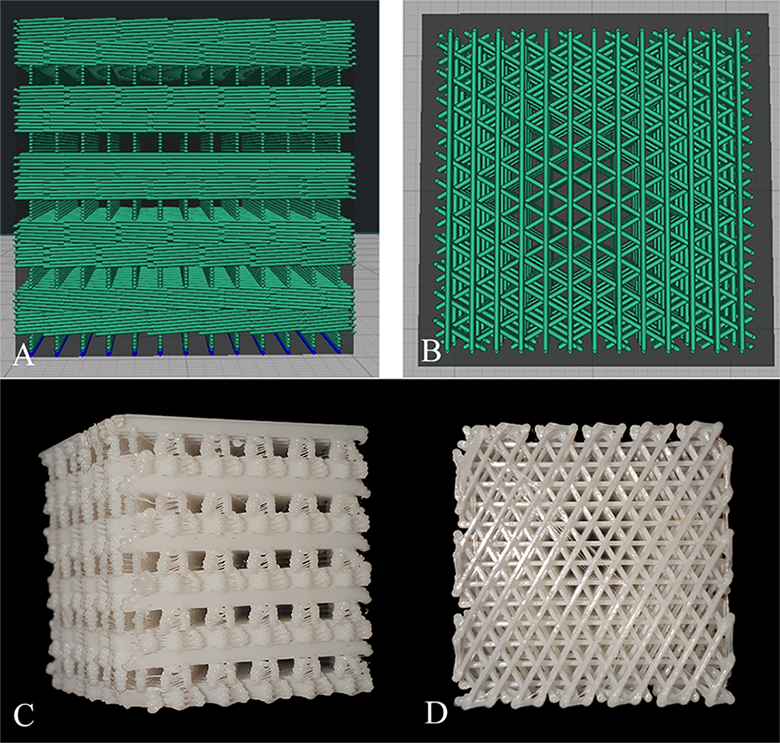
\includegraphics[width=0.9\textwidth, keepaspectratio]{mini_cube_full}
    \caption{\textbf{Scaffold in Cura}, \emph{Layer View}. Cubo 20mm per lato.
\textbf{A}: vista di fronte; \textbf{B}: vista da sopra;
\textbf{C} e \textbf{D}: scaffold stampato in PLA.
\textbf{Layer Height}: 0.2mm
\textbf{Layer Width}: 0.37mm
\textbf{Ugello diametro}: 0.4mm
\textbf{Infill Line Directions}: [0,0,0,0,0,0,60,60,60,60,60\-,60,60,120,120,120,120,120,120,120]
\textbf{Line Infill Distances}: \SI{1.52}{\milli\metre}.}
    \label{fig:mini_cube_full}
	\end{center}
\vspace{-20pt}
\end{figure}

\begin{figure}[t]
\vspace{-10pt}
	\begin{center}
	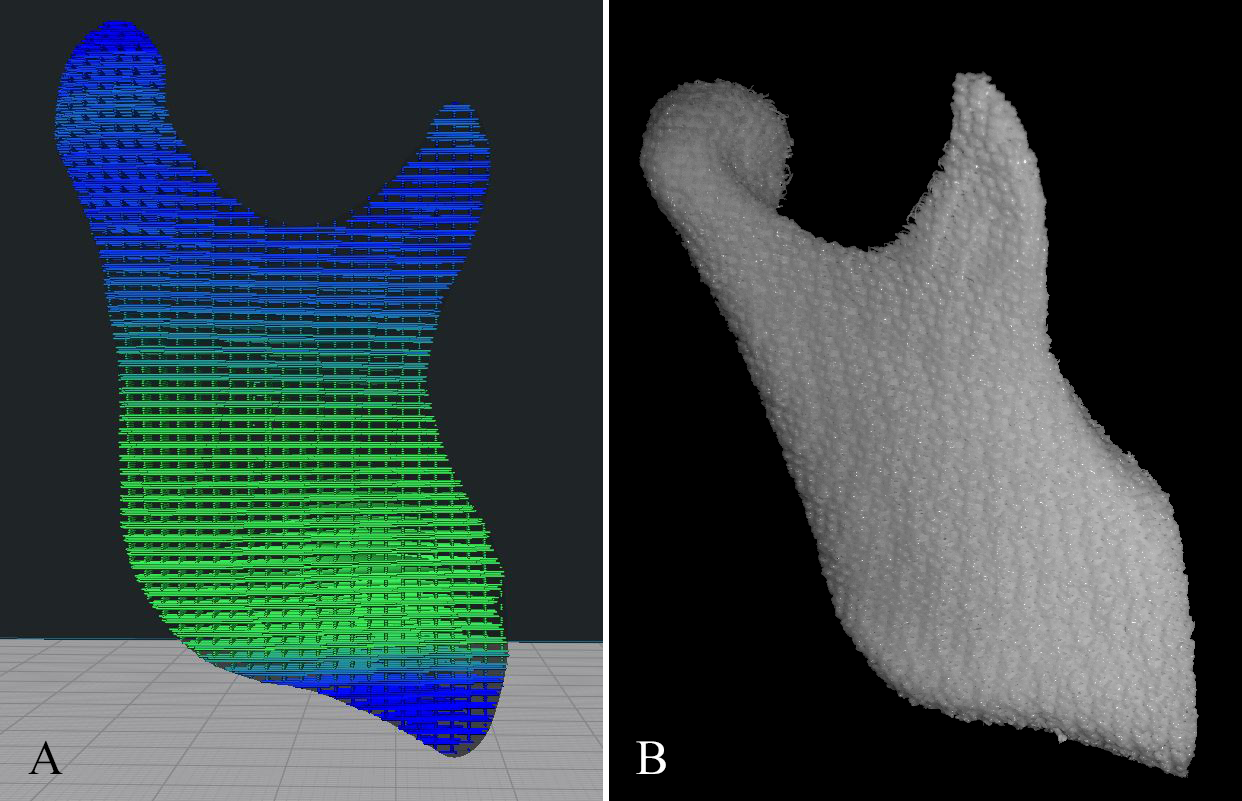
\includegraphics[width=0.9\textwidth, keepaspectratio]{scaffo_mandibola}
    \caption[LoF entry]{Scaffold derivato da un modello di ramo mandibolare.

\textbf{Layer Height}: 0.2mm
\textbf{Layer Width}: 0.37mm
\textbf{Ugello diametro}: 0.4mm
\textbf{Infill Line Directions}: [0,0,0,90,90,90]
\textbf{Line Infill Distances}: 0.8mm}
    \label{fig:scaffo_mandibola}
	\end{center}
\vspace{-20pt}
\end{figure}

